\newpage

\section{EAR - Eye Aspect Ratio} \label{section:EARsection}

Metoda polegająca na obliczeniu \textit{Eye Aspect Ratio} \cite{EARRaspberryPi} \cite{eyeBlinkEARRosebrock}, czyli stosunku otwarcia oczu - wysokość do szerokości widocznej części gałki ocznej. Wykorzystuje się tu znaczniki twarzy (rozdz.~\hyperref[{section:landmarks}]{\ref{section:landmarks}}) naniesione dookoła oczu.


\subsection{Wyznaczanie współczynnika EAR}

Zależnie od ilości punktów wokół oka wzór obliczania EAR może być różny.

\par

Dla 6 punktów:

\begin{align}
    EAR = \frac{dist(L_0, L_1) + dist(L_2, L4)}{2 * dist(L_3, L_5)}
\end{align}

Natomiast, dla 4 punktów:

\begin{align}
    EAR = \frac{dist(L_0, L_2)}{dist(L_1, L_3)}
\end{align}

Gdzie \textit{$L_x$} to kolejne znaczniki dokoła oczu, a~\textit{dist} to odległość między dwoma punktami (odległość euklidesowa).


\subsection{Zasada działania EAR w kontekście mrugania i~określenia czy oko jest otwarte/zamknięte}

W teorii otwarte oczy będą miały większy wymiar liczbowy EAR, niż oczy zamknięte. Na \hyperref[{fig:theoretical_eye_landmarks}]{rysunku \ref{fig:theoretical_eye_landmarks}} widać, że~oko otwarte ma większą odległości między punktami pionowymi niż w~przypadku oka zamkniętego. Dzięki takim różnicą możemy wykryć spadek wskaźnika EAR poniżej pewnego ustalonego poziomu, oznaczający zamknięcie oka. Natomiast wzrost, otwarcie oka. Całościowo obserwując zmiany np. za pomocą pochodnej jesteśmy w~stanie stwierdzić mrugnięcie.

\begin{figure}[!h]
    \begin{center}
        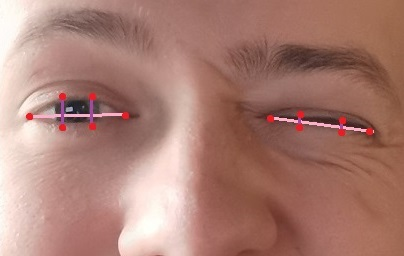
\includegraphics[scale=0.35]{img/landmark_section/theoretical_eye_landmarks.jpg}
        \caption{Teoretyczny rozmieszczenie znaczniki wokół oczu wraz z naniesionymi połączeniami punktów do obliczenia EAR.}
        \label{fig:theoretical_eye_landmarks}
    \end{center}
\end{figure}




\subsection{Ustalenie progu EAR}


Do skutecznego działania metod opartych na współczynniku EAR należało wyznaczyć próg wartości, poniżej którego oko klasyfikowane jest jako zamknięte. W~tym celu na potrzeby pracy dyplomowej zostały obliczone i~zebrane wartości EAR wykorzystując statyczne zdjęcia ze~zbioru danych oraz na podstawie obrazu z~kamery urządzenia. 


\subsubsection{EAR dla statycznych zdjęcia}

Na podstawie przygotowanego zbioru zdjęć został obliczony współczynnik EAR dla wszystkich oczu i~podzielony na dwie grupy: oczy otwarte (rys.~\ref{fig:ear_static_open}) i~oczy zamknięte (rys.~\ref{fig:ear_static_close}). 

\vspace{5mm}

\begin{figure}[!h]
    \centering
    \begin{tikzpicture}
        \begin{axis}[
            ylabel = {EAR},
            xlabel = {Numer zdjęcia oka},
            height = 0.4\linewidth,
            width = \linewidth,
            ymin= {0.10},
            ymax={0.40},
            ytick = {0.10, 0.15, 0.20, 0.25, 0.30, 0.35},
            ymajorgrids = {true},
        ]
            \addplot[color=blue, mark=square*, only marks] table [x=x, y=ear, col sep=comma] {csv/ear_static_open.csv};
        \end{axis}
    \end{tikzpicture}
    \caption{Rozkład  wartości współczynnika EAR oczu otwartych na zdjęciach ze zbioru danych.}
    \label{fig:ear_static_open}
\end{figure}

\begin{figure}[!h]
    \centering
    \begin{tikzpicture}
        \begin{axis}[
            ylabel = {EAR},
            xlabel = {Numer zdjęcia oka},
            height = 0.4\linewidth,
            width = 0.5\linewidth,
            ymin= {0.10},
            ymax={0.25},
            ytick = {0.1, 0.15, 0.2, 0.25},
            ymajorgrids = {true},
        ]
            \addplot[color=blue, mark=square*, only marks] table [x=x, y=ear, col sep=comma] {csv/ear_static_closed.csv};
        \end{axis}
    \end{tikzpicture}
    \caption{Rozkład  wartości współczynnika EAR oczu zamkniętych na zdjęciach ze zbioru danych.}
    \label{fig:ear_static_close}
\end{figure}

W przypadku oczu otwartych widać, że~poza kilkoma wyjątkami wskaźnik EAR znajduje się powyżej wartości $0.20$, a~czasem przekraczając nawet $0.35$. Przypadki gdzie wskazania są poniżej $0.15$ wynikają najprawdopodobniej z~faktu, że~oczy były mocno przymknięte i~ze względu na perspektywę rozciągnięte horyzontalnie. Odchylenie takie traktowane jest jako przypadek skrajny i~nie był brany pod uwagę w~końcowym doborze współczynnika.

\par

Na wykresie dla oczu zamkniętych ponownie próg zdaje się być na poziomie $0.20$, a~większość wskaźników osiąga wartość w przedziale $[0.15, 0.20]$. 



\subsubsection{EAR na obrazie z kamery}

Na obrazie z~kamery urządzenia przeprowadzone zostały trzy testy wskaźnika EAR: oczy otwarte (rys.~\ref{fig:ear_live_open}), oczy chwilowo zamknięte (rys.~\ref{fig:ear_live_close}) oraz mrugnięcie (rys.~\ref{fig:ear_live_blink}). Na~wykresach czerwony kolor oznacza wartość współczynnika dla prawego oka, natomiast niebieski dla lewego.


\begin{figure}[!h]
    \centering
    \begin{tikzpicture}
        \begin{axis}[
            xlabel = {Numer klatki obrazu z kamery},
            ylabel = {EAR},
            height = 0.4\linewidth,
            width = \linewidth,
            ymin= {0.20},
            ymax={0.35},
            ytick = {0.20, 0.25, 0.30, 0.35},
            ymajorgrids = {true},
        ]
            \addplot[color=blue, mark=square*] table [x=x, y=left, col sep=comma] {csv/ear_live_open.csv};
            \addplot[color=red, mark=square*] table [x=x, y=right, col sep=comma] {csv/ear_live_open.csv};
        \end{axis}
    \end{tikzpicture}
    \caption{Wartość współczynnika EAR dla oczu otwartych na obrazie z kamery.}
    \label{fig:ear_live_open}
\end{figure}

W przypadku gdy oczy były przez cały czas otwarte. Liczbowy wymiar EAR nie spadał poniżej $0.25$, a~przez większość czasu trzymał się nawet powyżej poziomu $0.30$.

\begin{figure}[!h]
    \centering
    \begin{tikzpicture}
        \begin{axis}[
            xlabel = {Numer klatki obrazu z kamery},
            ylabel = {EAR},
            height = 0.4\linewidth,
            width = \linewidth,
            ymin= {0.10},
            ymax={0.35},
            ytick = {0.15, 0.20, 0.25, 0.30, 0.35},
            ymajorgrids = {true},
        ]
            \addplot[color=blue, mark=square*] table [x=x, y=left, col sep=comma] {csv/ear_live_close.csv};
            \addplot[color=red, mark=square*] table [x=x, y=right, col sep=comma] {csv/ear_live_close.csv};
        \end{axis}
    \end{tikzpicture}
    \caption{Wartość współczynnika EAR dla oczu czasowo zamkniętych na obrazie z kamery.}
    \label{fig:ear_live_close}
\end{figure}

W~drugim teście oczy były czasowo zamknięte. Najpierw w~przedziale klatek $[25, 60]$ zamknięte było tylko oko prawe, następnie w~przedziale $[80,120]$ tylko lewe, a~na końcu w~okresie $[140,190]$ oba oczy jednocześnie. Zmiana EAR jest tutaj mocno wyraźna, a~w~tych trzech przedziałach wartość współczynnika wahała się między $0.10$, a~$0.20$. Dodatkowo na podstawie tych danych trzeba również odnotować spadek EAR dla obu oczu nawet w przypadku zamknięcia tylko jednego z~nich. Może to wynikać z~faktu, że~człowiek zamykając jedno oko przymyka lekko również drugie. Ale przyczyną może być też sam algorytm znaczników, w~którym punkty dla różnych oczu mogą być ze sobą skorelowane.

\begin{figure}[!h]
    \centering
    \begin{tikzpicture}
        \begin{axis}[
            xlabel = {Numer klatki obrazu z kamery},
            ylabel = {EAR},
            height = 0.4\linewidth,
            width = \linewidth,
            ymin= {0.10},
            ymax={0.35},
            ytick = {0.15, 0.20, 0.25, 0.30, 0.35},
            ymajorgrids = {true},
        ]
            \addplot[color=blue, mark=square*] table [x=x, y=left, col sep=comma] {csv/ear_live_blink.csv};
            \addplot[color=red, mark=square*] table [x=x, y=right, col sep=comma] {csv/ear_live_blink.csv};
        \end{axis}
    \end{tikzpicture}
    \caption{Wartość współczynnika EAR podczas mrugania na obrazie z kamery.}
    \label{fig:ear_live_blink}
\end{figure}

W~ostatniej wariacji testu na obrazie z~kamery występowały mrugnięcia: w~przedziale $[30,40]$ prawego oka, $[55,65]$ lewego, a~w~przedziale $[80,90]$ oboma oczami na raz. Szybka zmiana wymiaru EAR jest w~tych chwilach bardzo wyraźna i~łatwa do wykrycia. W~szczytowych chwilach mrugnięcia wartość spadała prawie do poziomu $0.15$. Ponownie występuje tu zmniejszenie EAR dla obu oczu nawet w~przypadku mrugnięcia wyłącznie jednym. 


\subsection{Wnioski}

Zmiany wartości EAR na obrazie z~kamery są bardzo wyraźne i~łatwe do wykrycia. Dzięki temu metoda ta nadaje się do detekcji mrugania i~tego czy oczy są zamknięte. 

\vspace{3mm}

Na podstawie testów progowy poziom EAR dla oka zamkniętego ustalony został na $\leq0.19$. Powyżej tej wartości oko traktowane jest jako otwarte. 

\vspace{3mm}

Jednak problem ze zmianą EAR dla obu oczu nawet w przypadku zamykania tylko jednego z~nich sprawia, że~w~finalnej wersji pracy dyplomowej odnotowywany jest wyłącznie fakt mrugnięcia bez podziału na to którym okiem została wykonana czynność.
